\documentclass[border=15pt]{standalone}
\usepackage{amsmath, amssymb}
\usepackage{tikz}
\usetikzlibrary{arrows.meta}

\definecolor{block0}{HTML}{E53935}
\definecolor{block1}{HTML}{1E88E5}
\definecolor{block2}{HTML}{43A047}

\begin{document}
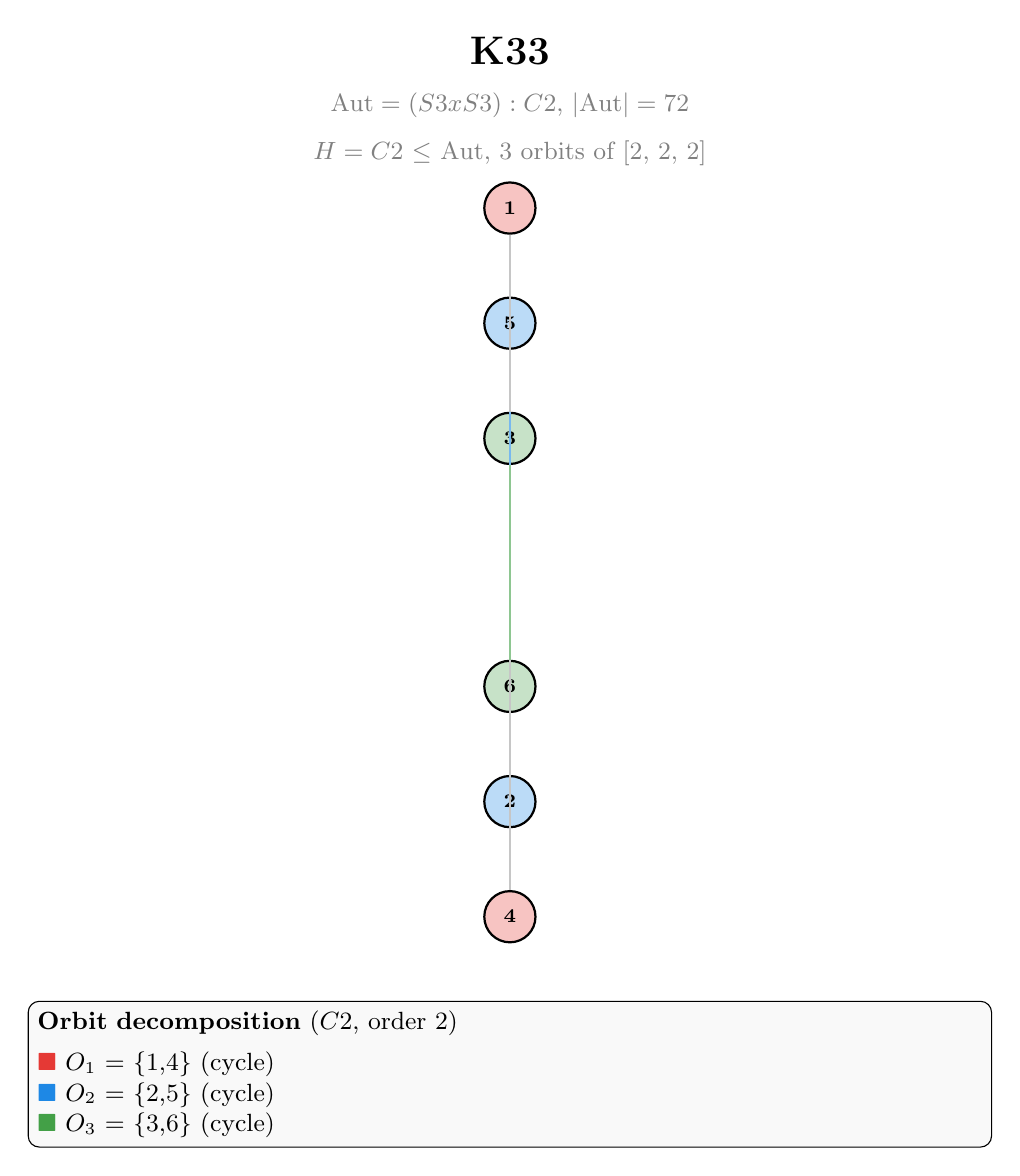
\begin{tikzpicture}[
  vertex/.style={circle, draw, thick, minimum size=6.5mm, inner sep=0pt,
                 font=\scriptsize\bfseries},
  edge/.style={thick, gray!45},
  title/.style={font=\Large\bfseries},
  subtitle/.style={font=\small, text=gray},
]

\node[title] at (0, 6.5) {K33};
\node[subtitle] at (0, 5.8) {$\mathrm{Aut} = (S3 x S3) : C2$, $|\mathrm{Aut}| = 72$};
\node[subtitle] at (0, 5.2) {$H = C2$ $\leq$ $\mathrm{Aut}$, 3 orbits of [2, 2, 2]};

\node[vertex, fill=block0!30] (v1) at (0.000, 4.500) {1};
\node[vertex, fill=block1!30] (v2) at (-0.000, -3.038) {2};
\node[vertex, fill=block2!30] (v3) at (0.000, 1.575) {3};
\node[vertex, fill=block0!30] (v4) at (-0.000, -4.500) {4};
\node[vertex, fill=block1!30] (v5) at (0.000, 3.038) {5};
\node[vertex, fill=block2!30] (v6) at (-0.000, -1.575) {6};

\draw[thick, block0!60] (v1) -- (v4);
\draw[edge] (v1) -- (v5);
\draw[edge] (v1) -- (v6);
\draw[edge] (v2) -- (v4);
\draw[thick, block1!60] (v2) -- (v5);
\draw[edge] (v2) -- (v6);
\draw[edge] (v3) -- (v4);
\draw[edge] (v3) -- (v5);
\draw[thick, block2!60] (v3) -- (v6);

\node[draw, rounded corners, fill=gray!5, text width=12cm, align=left, font=\small]
  at (0, -6.5) {
  \textbf{Orbit decomposition} ($C2$, order 2) \\[4pt]
  \textcolor{block0}{$\blacksquare$} $O_{1}$ = \{1,4\} (cycle) \\
  \textcolor{block1}{$\blacksquare$} $O_{2}$ = \{2,5\} (cycle) \\
  \textcolor{block2}{$\blacksquare$} $O_{3}$ = \{3,6\} (cycle)
};

\end{tikzpicture}
\end{document}